\subsubsection{Digit tops}
The {\dtop} gadgets have special geometry designed so that {\firstwarp} and
{\secondwarp} tiles are allowed to ``wake up", and complete their warping journey. Each
digit has some type of {\dtop} gadget, however, depending on the digit region
and index of a specific digit, the exact digit top will differ.

% talk about geometry of digit tops enabling first and second warp tiles to "wake up"

\vspace{.5cm}


\begin{figure}[H]
    \centering
    \begin{subfigure}[t]{0.32\textwidth}
        \centering
        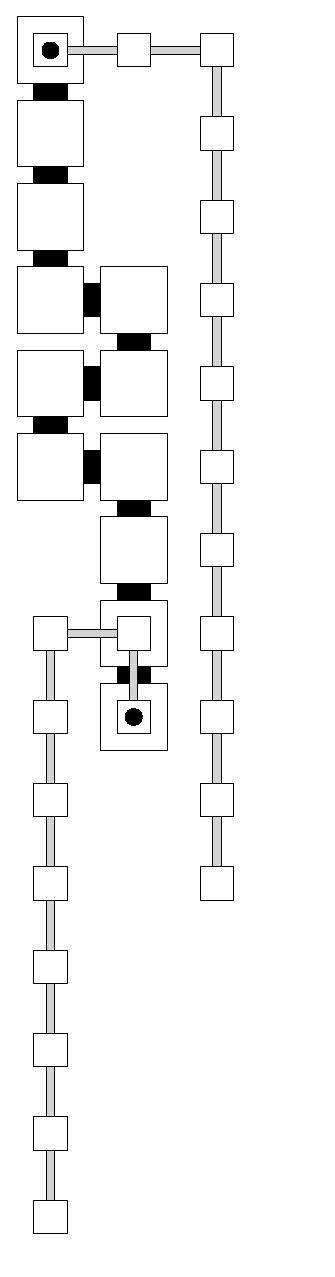
\includegraphics[width=0.32\textwidth]{digit_top_general_topper}
        \caption{\label{fig:topper_gen} General topper}
    \end{subfigure}%
    ~
    \begin{subfigure}[t]{0.32\textwidth}
        \centering
        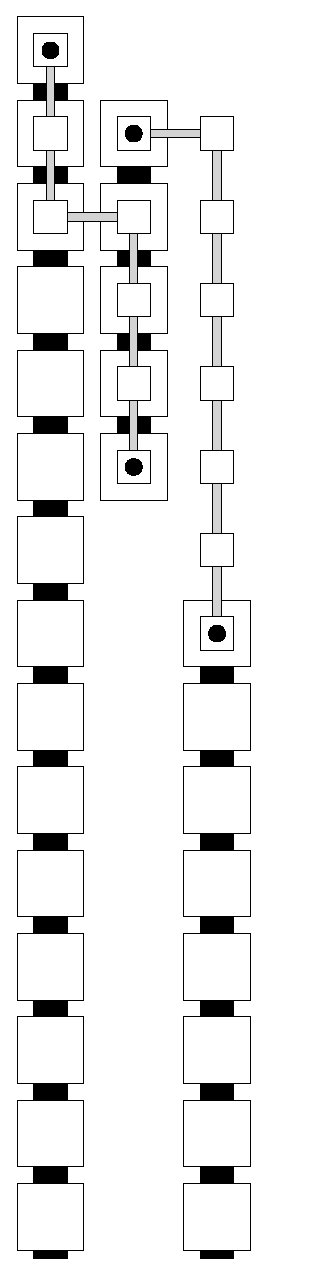
\includegraphics[width=0.32\textwidth]{digit_top_case1_digit1_topper}
        \caption{\label{fig:topper_case1} Case 1 -- topper}
    \end{subfigure}%
    ~
    \begin{subfigure}[t]{0.32\textwidth}
        \centering
        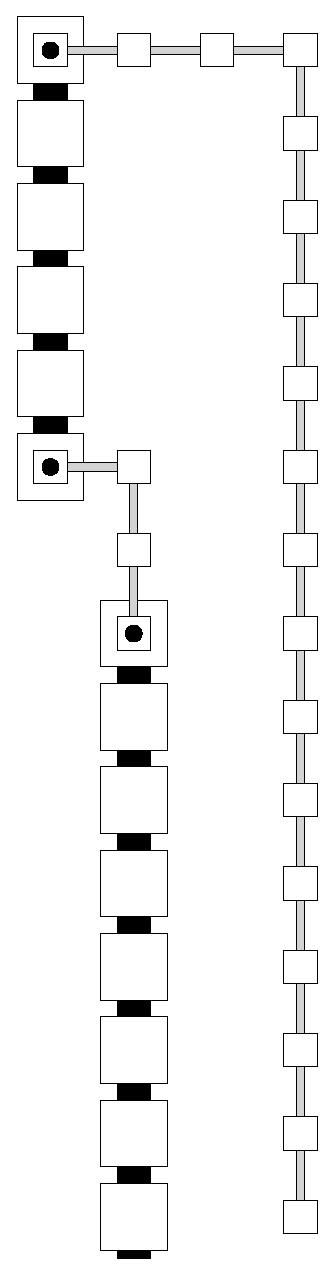
\includegraphics[width=0.32\textwidth]{digit_top_case2_digit2_topper}
        \caption{\label{fig:topper_case2} Case 2 -- topper}
    \end{subfigure}%
    \caption{\label{fig:topper_microgadgets} Topper micro-gadgets }
\end{figure}


For each $\inc \in \{ {\tt increment, copy } \}$
    \begin{itemize}

        \item Digit 1 (general): the following statements create the gadget shown in Figure~\ref{fig:digit_top_general}
        \begin{itemize}
            \item Create
            $\begin{aligned}[t]
                {\tt North\_Line5}(& \left \langle {\tt DigitTop},  1, \inc \right\rangle,
                                     \left \langle {\tt DigitTopA}, 1, \inc \right\rangle \;)
            \end{aligned}$\\from the micro-gadget shown in Figure~\ref{fig:north_line}.

            \item Create
            $\begin{aligned}[t]
                {\tt Topper}(& \left \langle {\tt DigitTopA}, 1, \inc \right\rangle,
                               \left \langle {\tt DigitTopB}, 1, \inc \right\rangle \;)
            \end{aligned}$\\from the micro-gadget shown in Figure~\ref{fig:topper_gen}.

            \item Create
            $\begin{aligned}[t]
                {\tt South\_Line4\textit{l}}(& \left\langle {\tt DigitTopB}, 1, \inc \right\rangle,
                                               \left\langle \returnpath,     1, \inc \right\rangle \;)
            \end{aligned}$\\from the micro-gadget shown in Figure~\ref{fig:south_line}.
        \end{itemize}
        \vspace{1cm}

        \item Digit 1 (MSR): the following statements create the gadget shown in Figure~\ref{fig:digit_top_case2_digit1_msr}
        \begin{itemize}
            \item Create
            $\begin{aligned}[t]
                {\tt Topper}(& \left\langle {\tt DigitTop},  1, \inc, {\tt msr} \right\rangle,
                               \left\langle {\tt DigitTopA}, 1, \inc, {\tt msr} \right\rangle \;)
            \end{aligned}$ \\ from the micro-gadget shown in Figure~\ref{fig:topper_case1}.


            \item Create
            $\begin{aligned}[t]
                {\tt South\_Line4\textit{l}}(& \left\langle {\tt DigitTopA}, 1, \inc, {\tt msr}\right\rangle,
                                               \left\langle \returnpath,     1, \inc, {\tt msr}\right\rangle \;)
            \end{aligned}$ \\ from the micro-gadget shown in Figure~\ref{fig:south_line}.
        \end{itemize}
        \vspace{1cm}


        \item Digit 1 (MSD): the following statements create the gadget shown in Figure~\ref{fig:digit_top_case1_digit1_msr}
        \begin{itemize}
            \item Create
            $\begin{aligned}[t]
                {\tt North\_Line4\textit{l}}(& \left\langle {\tt DigitTop},  1, \inc, {\tt msr}, {\tt msd}\right\rangle,
                                               \left\langle {\tt DigitTopA}, 1, \inc, {\tt msr}, {\tt msd}\right\rangle \;)
            \end{aligned}$\\from the micro-gadget shown in Figure~\ref{fig:north_line}.

            \item Create $\begin{aligned}[t]
                {\tt North\_Line4}(& \left\langle {\tt DigitTopA}, 1, \inc, {\tt msr}, {\tt msd}\right\rangle,
                                     \left\langle {\tt DigitTopB}, 1, \inc, {\tt msr}, {\tt msd}\right\rangle \;)
            \end{aligned}$\\from the micro-gadget shown in Figure~\ref{fig:north_line}.

            \item Create $\begin{aligned}[t]
                {\tt Topper}(& \left\langle {\tt DigitTopB}, 1, \inc, {\tt msr}, {\tt msd}\right\rangle,
                               \left\langle {\tt DigitTopC}, 1, \inc, {\tt msr}, {\tt msd}\right\rangle \;)
            \end{aligned}$\\from the micro-gadget shown in Figure~\ref{fig:topper_gen}.

            \item Create
            $\begin{aligned}[t]
                {\tt South\_Line4\textit{l}}(& \left\langle {\tt DigitTopC}, 1, \inc, {\tt msr}, {\tt msd}\right\rangle,
                                               \left\langle {\tt DigitTopD}, 1, \inc, {\tt msr}, {\tt msd}\right\rangle \;)
            \end{aligned}$\\from the micro-gadget shown in Figure~\ref{fig:south_line}.

            \item Create
            $\begin{aligned}[t]
                {\tt South\_Line30}(& \left\langle {\tt DigitTopD}, 1, \inc, {\tt msr}, {\tt msd}\right\rangle,
                                      \left\langle {\tt DigitTopE}, 1, \inc, {\tt msr}, {\tt msd}\right\rangle \;)
            \end{aligned}$\\from the micro-gadget shown in Figure~\ref{fig:south_line}.

            \item Create
            $\begin{aligned}[t]
                {\tt South\_Line4\textit{l}}(& \left\langle {\tt DigitTopE}, 1, \inc, {\tt msr}, {\tt msd}\right\rangle,
                                               \left\langle {\tt DigitTopF}, 1, \inc, {\tt msr}, {\tt msd}\right\rangle \;)
            \end{aligned}$\\ from the micro-gadget shown in Figure~\ref{fig:south_line}.

            \item Create
            $\begin{aligned}[t]
                {\tt South\_Line14}(& \left\langle {\tt DigitTopF}, 1, \inc, {\tt msr}, {\tt msd}\right\rangle,
                                      \left\langle {\tt DigitTopG}, 1, \inc, {\tt msr}, {\tt msd}\right\rangle \;)
            \end{aligned}$\\ from the micro-gadget shown in Figure~\ref{fig:south_line}.

            \item Create
            $\begin{aligned}[t]
                {\tt South\_Line17}(& \left\langle {\tt DigitTopG}, 1, \inc, {\tt msr}, {\tt msd} \right\rangle,
                                      \left\langle \returnpath,     1, \inc, {\tt msr}, {\tt msd} \right\rangle \;)
            \end{aligned}$\\from the micro-gadget shown in Figure~\ref{fig:south_line}.
        \end{itemize}
        \vspace{1cm}


        \item Digit 2 (general): the following statements create the gadget shown in Figure~\ref{fig:digit_top_general}
        \begin{itemize}
            \item Create
            $\begin{aligned}[t]
                {\tt North\_Line5}(& \left\langle {\tt DigitTop}, 2, \inc \right\rangle,
                                     \left\langle {\tt DigitTopA} 2, \inc \right\rangle \;)
            \end{aligned}$\\from the micro-gadget shown in Figure~\ref{fig:north_line}.

            \item Create
            $\begin{aligned}[t]
                {\tt Topper}(& \left\langle {\tt DigitTopA} 2, \inc \right\rangle,
                               \left\langle {\tt DigitTopB} 2, \inc \right\rangle \;)
            \end{aligned}$\\from the micro-gadget shown in Figure~\ref{fig:topper_gen}.

            \item Create
            $\begin{aligned}[t]
                {\tt South\_Line4\textit{l}}(& \left\langle {\tt DigitTopB} 2, \inc \right\rangle,
                                               \left\langle \returnpath,    2, \inc \right\rangle \;)
            \end{aligned}$\\from the micro-gadget shown in Figure~\ref{fig:south_line}.
        \end{itemize}
        \vspace{1cm}


        \item Digit 2 (MSD): the following statements create the gadget shown in Figure~\ref{fig:digit_top_case2_digit2_msr}
        \begin{itemize}
            \item Create
            $\begin{aligned}[t]
                {\tt North\_Line4\textit{l}}(& \left\langle {\tt DigitTop},  2, \inc, {\tt msr}, {\tt msd} \right\rangle,
                                               \left\langle {\tt DigitTopA}, 2, \inc, {\tt msr}, {\tt msd} \right\rangle\;)
            \end{aligned}$\\ from the micro-gadget shown in Figure~\ref{fig:north_line}.

            \item Create
            $\begin{aligned}[t]
                {\tt Topper}(& \left\langle {\tt DigitTopA}, 2, \inc, {\tt msr}, {\tt msd} \right\rangle,
                               \left\langle {\tt DigitTopB}, 2, \inc, {\tt msr}, {\tt msd} \right\rangle \;)
            \end{aligned}$\\from the micro-gadget shown in Figure~\ref{fig:topper_case2}.

            \item Create
            $\begin{aligned}[t]
                {\tt South\_Line4\textit{l}}(& \left\langle {\tt DigitTopB}, 2, \inc, {\tt msr}, {\tt msd} \right\rangle,
                                               \left\langle {\tt DigitTopC}, 2, \inc, {\tt msr}, {\tt msd} \right\rangle \;)
            \end{aligned}$\\from the micro-gadget shown in Figure~\ref{fig:south_line}.

            \item Create
            $\begin{aligned}[t]
                {\tt South\_Line30}(& \left\langle {\tt DigitTopC}, 2, \inc, {\tt msr}, {\tt msd} \right\rangle,
                                      \left\langle \returnpath,     2, \inc, {\tt msr}, {\tt msd}\right\rangle \;)
            \end{aligned}$\\from the micro-gadget shown in Figure~\ref{fig:south_line}.
        \end{itemize}
        \vspace{1cm}


        \item Digit 3 (general): the following statements create the gadget from Figure~\ref{fig:digit_top_general}
        \begin{itemize}
            \item Create
            $\begin{aligned}[t]
                {\tt North\_Line5}(& \left\langle {\tt DigitTop},  3, \inc \right\rangle,
                                     \left\langle {\tt DigitTopA}, 3, \inc \right\rangle \;)
            \end{aligned}$\\from the micro-gadget shown in Figure~\ref{fig:north_line}.

            \item Create
            $\begin{aligned}[t]
                {\tt Topper}(& \left\langle {\tt DigitTopA}, 3, \inc  \right\rangle,
                               \left\langle {\tt DigitTopB}, 3, \inc  \right\rangle \;)
            \end{aligned}$\\from the micro-gadget shown in Figure~\ref{fig:topper_gen}.

            \item Create
            $\begin{aligned}[t]
                {\tt South\_Line4\textit{l}}(& \left\langle {\tt DigitTopB}, 3, \inc \right\rangle,
                                               \left\langle \returnpath,     3, \inc \right\rangle \;)
            \end{aligned}$\\from the micro-gadget shown in Figure~\ref{fig:south_line}.
        \end{itemize}
        \vspace{1cm}


        \item Digit 3 (MSD): the following statements create the gadget from Figure~\ref{fig:digit_top_general}
        \begin{itemize}
            \item Create
            $\begin{aligned}[t]
                {\tt North\_Line5}(& \left\langle {\tt DigitTop},  3, \inc, {\tt msr}, {\tt msd}\right\rangle,
                                     \left\langle {\tt DigitTopA}, 3, \inc, {\tt msr}, {\tt msd}\right\rangle \;)
            \end{aligned}$\\from the micro-gadget shown in Figure~\ref{fig:north_line}.

            \item Create
            $\begin{aligned}[t]
                {\tt Topper}(& \left\langle {\tt DigitTopA}, 3, \inc, {\tt msr}, {\tt msd}\right\rangle,
                               \left\langle {\tt DigitTopB}, 3, \inc, {\tt msr}, {\tt msd}\right\rangle \;)
            \end{aligned}$\\ from the micro-gadget shown in Figure~\ref{fig:topper_gen}.


            \item Create
            $\begin{aligned}[t]
                {\tt South\_Line4\textit{l}}(& \left\langle {\tt DigitTopB}, 3, \inc, {\tt msr}, {\tt msd}\right\rangle,
                                               \left\langle \returnpath,     3, \inc, {\tt msr}, {\tt msd}\right\rangle \;)
            \end{aligned}$\\ from the micro-gadget shown in Figure~\ref{fig:south_line}.
        \end{itemize}

    \end{itemize}


    \begin{figure}[H]
        \centering
        \begin{subfigure}[t]{0.24\textwidth}
            \centering
            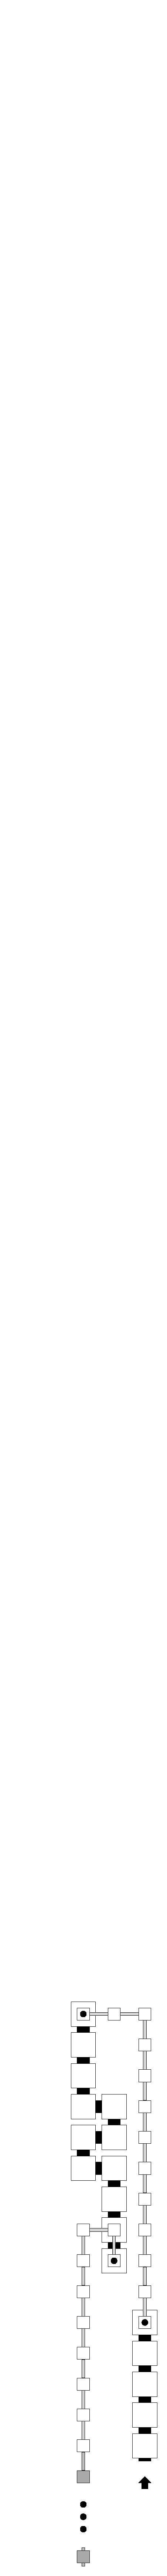
\includegraphics[width=0.245\textwidth]{digit_top_general}
            \caption{\label{fig:digit_top_general} General}
        \end{subfigure}%
        ~
        \begin{subfigure}[t]{0.24\textwidth}
            \centering
            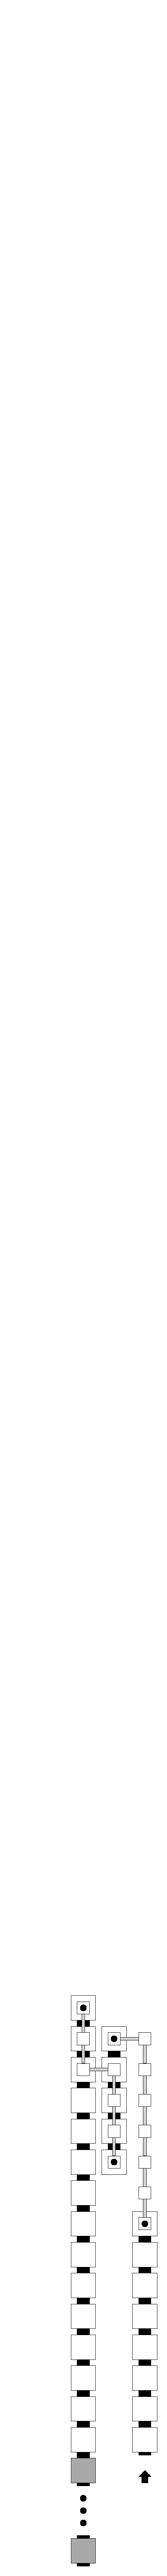
\includegraphics[width=0.245\textwidth]{digit_top_case2_digit1_msr}
            \caption{\label{fig:digit_top_case2_digit1_msr} Digit 1 -- Case 2}
        \end{subfigure}%
        ~
    \end{figure}

    \begin{figure}[H]\ContinuedFloat
        \centering
        \begin{subfigure}[t]{0.24\textwidth}
            \centering
            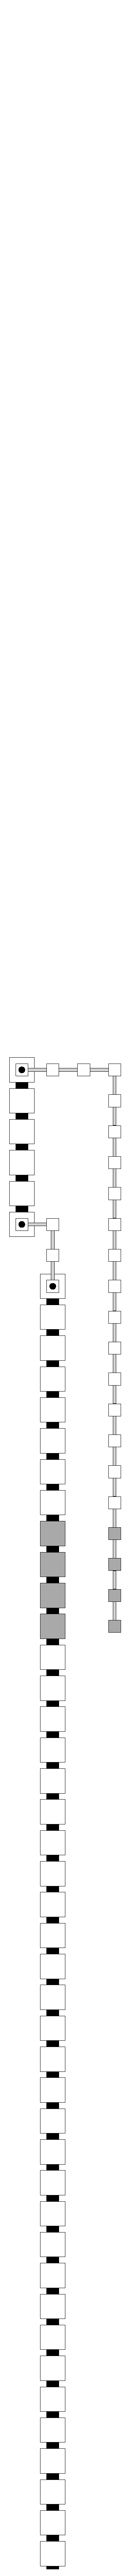
\includegraphics[width=0.245\textwidth]{digit_top_case2_digit2_msr}
            \caption{\label{fig:digit_top_case2_digit2_msr} Digit 2 -- Case 2}
        \end{subfigure}%
        ~
        \begin{subfigure}[t]{0.24\textwidth}
            \centering
            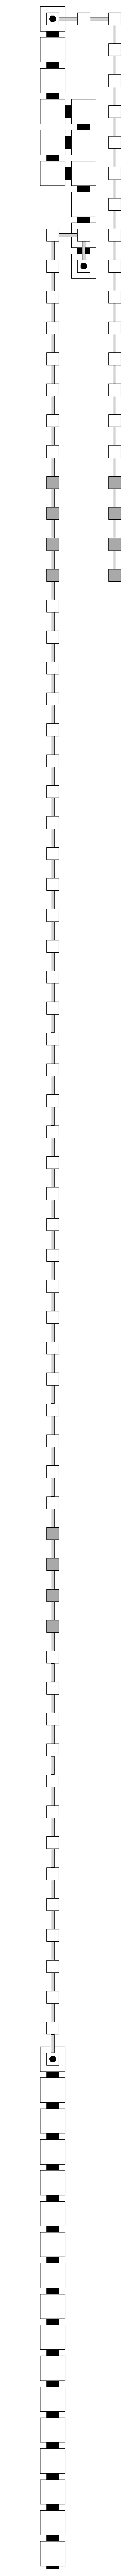
\includegraphics[width=0.245\textwidth]{digit_top_case1_digit1_msr}
            \caption{\label{fig:digit_top_case1_digit1_msr} Digit 1 -- Case 1}
        \end{subfigure}%
        ~
        \caption{\label{fig:digit_tops} {\tt Digit\_Top} gadgets}
    \end{figure}

\vspace{1cm}
